\documentclass[a5paper,oneside]{amsart}
\usepackage[scale={.9,.9}]{geometry}
\usepackage{mathrsfs}
\usepackage{listings}
\usepackage{dsfont}
\usepackage{graphicx}
\theoremstyle{plain}
\newtheorem{theorem}{Theorem}
\newtheorem{lemma}{Lemma}
\newtheorem{corollary}{Corollary}
\newtheorem{proposition}{Proposition}
\newtheorem{conjecture}{Conjecture}
\theoremstyle{definition}
\newtheorem{problema}{Problema}
\newtheorem{ejercicio}{Ejercicio}
\newtheorem*{definition}{Definition}
\newtheorem*{remark}{Remark}
\usepackage{listings}
\lstset{
language=R,
basicstyle=%\scriptsize
\ttfamily,
commentstyle=\ttfamily\color{gray},
numbers=none,
numberstyle=\ttfamily\color{gray}\footnotesize,
stepnumber=1,
numbersep=5pt,
backgroundcolor=\color{white},
showspaces=false,
showstringspaces=false,
showtabs=false,
frame=none,
tabsize=4,
captionpos=b,
breaklines=true,
breakatwhitespace=false,
title=\lstname,
escapeinside={},
keywordstyle={},
morekeywords={}
}
\title[Problemas de Procesos I]{Problemas de Procesos Estoc\'asticos I\\ Semestre 2013-II\\ Posgrado en Ciencias Matem\'aticas\\ Universidad Nacional Aut\'onoma de M\'exico\\ TAREA 2}
\author{Antonio Soriano Flores}
%\address{}
\usepackage[colorlinks,citecolor=blue,urlcolor=blue]{hyperref}
\input{definitions.tex}
%\usepackage[colorlinks,citecolor=blue,urlcolor=blue]{hyperref}
\begin{document}
\maketitle




\begin{problema}
Sea \(S_n=X_1+\cdots+X_n\) una caminata aleatoria con saltos \(X_i\in \{-1,0,1,\ldots\}\). Sea \(C_p\) una variable aleatoria geom\'etrica de par\'ametro \(p\) independiente de \(S\) y definimos $$ M_p=-\min_{n\leq C_p} S_n. $$El objetivo del ejercicio es determinar la distribuci\'on de \(M_p\).

(A las caminatas aleatorias como \(S\) se les ha denominado Skip-free random walks Para aplicaciones de este tipo de procesos, ver \cite{MR1978607}. Tambi\'en aparecen en el estudio de Procesos Galton-Watson. Este ejercicio es el resultado b\'asico del estudio de sus extremos, denominado teor\'ia de fluctuaciones.)

\begin{enumerate}
\item Sea$$g(\lambda)=E(e^{- \lambda X_1}).$$Pruebe que \(g(\lambda)\in (0,\infty)\) y que$$M_n=e^{-\lambda S_n}g(\lambda)^{-n},n\geq 0$$es una martingala.
\begin{proof}
Como:
$$
e^{-\lambda X_1}>0 \Rightarrow \esp{e^{-\lambda X_1}}>0 \Rightarrow g(\lambda)>0
$$
Ademas
$$
-1\leq X_1\Rightarrow \lambda \geq -\lambda X_1 \Rightarrow e^{\lambda} \geq e^{-\lambda X_1} \Rightarrow  \esp{e^{\lambda}}\geq  \esp{e^{-\lambda X_1}}  \Rightarrow g(\lambda) \leq e^{\lambda}
$$
Concluimos entonces que:
$$
0\leq g(\lambda)\leq e^{\lambda} \Rightarrow g(\lambda) \in (0,\infty)
$$
Ahora probaremos que $M_n$ as\'i definida es martingala
\begin{itemize}
	\item. $M_n$ es $\F_n$-medible  (Suponemos que $\F_n=\sigma(X_1,X_2,...,X_n)$)  pues  $S_n$ es funci\'on medible de $X_1,X_2,...,X_n$
	$$
	S_n=f(X_1,X_2,...,X_n)=X_1+X_2+....+X_n
	$$  
	\item $M_n\in L_1$ pues sabemos que $g(\lambda)=\esp{e^{- \lambda X_1}}\leq e^\lambda \leq \infty$ entonces:
	$$
	M_n=e^{-\lambda S_n}g(\lambda)^{-n}=g(\lambda)^{-n}\prod_{i=1}^{n}e^{-\lambda X_i}
	$$
	Entonces $M_n$ es producto finito de variables en $L_1$ y como las variables son independientes se sigue que $M_n \in L_1$
	\item Demostraremos que $\esp{M_{n+1}|\F_n}=M_n$.
	$$
	\esp{M_{n+1}|\F_n}=\esp{e^{-\lambda S_{n+1}}g(\lambda)^{-(n+1)}|\F_n}
	$$
	$$
	=g(\lambda)^{-(n+1)}\esp{e^{-\lambda S_n}e^{-\lambda X_{n+1}}|\F_n}=g(\lambda)^{-(n+1)}e^{-\lambda S_n}\esp{e^{-\lambda X_{n+1}}}
	$$
	$$
	=g(\lambda)^{-(n+1)}e^{-\lambda S_n}\esp{e^{-\lambda X_{1}}}=g(\lambda)^{-(n+1)}e^{-\lambda S_n}g(\lambda)=M_n
	$$
	Observaci\'on. Aqu\'i utilizamos propiedades de la esperanza condicional y que $S_n$ es $\F_n$-medible as\'i como la independencia que hay entre las variables $X_i$. Dado que estamos utilizando esperanzas condicionales, las igualdades anteriores deben de tomarse como casi-seguramente. 
	
\end{itemize}
Por los tres puntos anteriores se concluye que $M_n$ es martingala
	
\end{proof}
\item Pruebe que \(g\) es log-convexa al aplicar la desigualdad de H\"older. Pruebe que si \(P(X_1=-1)>0\) (hip\'otesis que se utilizar\'a desde ahora) entonces \(g(\lambda)\to\infty\) conforme \(\lambda\to\infty\). Utilice esta informaci\'on para esbozar la gr\'afica de \(g\). Defina \( f(s)=\inf \{ \lambda>0:g(\lambda)^{-1} < s\} \). Note que \(1/g\circ f=Id\) en \((0,1)\). Pruebe que si \(g(\lambda)>1\), la martingala \(M\) es acotada hasta el tiempo de arribo de \(S\) a \(-k\) dado por $$ T_k =\min \{n\in\na:S_n=-k\} $$(donde se utiliza la convenci\'on \(\inf\emptyset=\infty\) ). Aplique el teorema de muestreo opcional de Doob para mostrar que$$E(s^{T_k})=e^{-k f(s)} .$$Justifique MUY bien por qu\'e la f\'ormula es v?lida aun cuando \(T_k\) puede tomar el valor \(\infty\) y deduzca que de hecho \(\p (T_k=\infty)=0\).
\begin{proof}
Necesitamos probar que $log(g(\lambda))$ es convexa. Hay que probar entonces que para cualesquiera $a$ y $b$ en el dominio de $g$ se tiene que para toda $t \in (0,1)$:
$$
log(g(a(1-t)+bt)) \leq log(g(a))(1-t)+log(g(b))t 
$$
Rercordando la definici�n de $g$ tenemos que:
$$
log(g(a(1-t)+bt))=log\paren{\esp{e^{-(a(1-t)+bt)X_1}}}=log\paren{\esp{e^{-a(1-t)X_1}e^{-btX_1}}}
$$
Sea $p=\frac{1}{1-t}$ y $q=\frac{1}{t}$. Entonces $\frac{1}{p}+\frac{1}{q}=1$. Entonces bajo estas definici\'on podemos asegurar que:
$$
e^{-a(1-t)X_1} \in L_p \text{  y  }  e^{-btX_1} \in L_q
$$
Por lo tanto usando la desigualdad de H�lder:
$$
\esp{e^{-a(1-t)X_1}e^{-btX_1}}\leq \esp{e^{-a(1-t)X_{1}p}}^{\frac{1}{p}} \esp{e^{-btX_{1}q}}^{\frac{1}{q}}
$$
$$
=\esp{e^{-aX_{1}}}^{1-t} \esp{e^{-bX_{1}}}^{t}=g(a)^{1-t}g(b)^{t}
$$
Tomando logaritmo (funci\'on creciente) obtenemos:
$$
log(\esp{e^{-a(1-t)X_1}e^{-btX_1}})\leq log(g(a)^{1-t}g(b)^{t})=(1-t)log(g(a))+tlog(g(b))
$$
Por lo tanto
$$
log(g(a(1-t)+bt)) \leq log(g(a))(1-t)+log(g(b))t 
$$
De donde se sigue que $g$ es log-convexa.\\
Observaci\'on: 
\begin{itemize}
	\item $g$ tambi\'en es convexa pues $g=e^{(log(g))}$ donde sabemos que la funci\'on exponencial es convexa y creciente. (Aqu\'i hay que recordar que la composici\'on  de una funci\'on convexa con otra convexa y creciente genera una funci\'on convexa).
	\item $g$ es continua. Pues sea $\set{X_n}$ una sucesi\'on de reales en $(0,\infty)$ que converge a $X_0$ entonces $g(X_n)$ converge a $g(X_0)$. Lo anterior es porque podemos intercambiar el limite con esperanza ya que la sucesi\'on  $\set{g(X_n)}$ es dominada. Esto ultimo porque: $g(X_n)\leq e^{X_n}$ (recordar que en el inciso anterior probamos que $g(\lambda)\leq e^\lambda$) y como $X_n$ es convergente entonces es acotada, luego entonces existe $X_*$ tal que $ e^{X_n}\leq e^{X_*}$ para toda n, de donde se sigue que  $\set{g(X_n)}$ es dominada y por tanto se puede utilizar T.C.D de donde se concluye que en efecto $g(X_n)$ converge a $g(X_0)$. Lo que a su vez muestra la continudad de $g$.
\end{itemize}

Ahora supongamos que $\p(X=-1)>0$. Utilizando el teorema de cambio de variable para calcular la esperanza:
$$
g(\lambda)=\esp{e^{-\lambda X_1}}=\sum_{i=-1}^{\infty}e^{-\lambda i}\p(X=i)\leq e^{\lambda}\p(X=-1)
$$
Por lo tanto hemos probado que:
$$
 e^{\lambda}\p(X=-1)\leq g(\lambda)
$$\\
De donde se observa que si $\lambda$ tiene a infinito, entonces $g(\lambda)$ tambi\'en crece a infinito.

Es decir una cota inferior para la funci\'on $g(\lambda)$ es   $e^{\lambda}\p(X=-1)$\\
Por otro lado, se define $f(s)=inf\set{\lambda > 0: g(\lambda)^{-1}<s}$.  Sea $s \in (0,1)$ y supongamos que $a=f(s)$ entonces por definici�n de infimo $a$ es una cota inferior  luego entonces para toda $n$
$$
\frac{1}{s} < g\paren{a+\frac{1}{n}} 
$$
Por lo que tomando limite y usando la continuidad de $g$:
$$
\frac{1}{s} \leq g\paren{a}
$$
Demostraremos que $\frac{1}{s} = g\paren{a}$ por contradicci\'on. Supongamos que $\frac{1}{s} > g\paren{a}$, entonces por la continuidad de $g$ sabemos que existe una vecindad al rededor de $a$ tal que  para toda $x$ en esa vecindad  $g(x)>\frac{1}{s}$. Es decir, existe $\eps$ tal que para toda $x \in \set{|x-a|<\eps}$ se  tiene que   $g(x)>\frac{1}{s}$. tomemos $x_*=a-\eps/2$. Entonces tendri\'amos que  (como $x_* \in\set{\lambda > 0: g(\lambda)^{-1}<s}$)
$$
a\leq x_*=a-\eps/2 < a 
$$
Lo que nos lleva a una contradicci\'on.\\ Por lo tanto  $\frac{1}{s} = g\paren{a}$ , pero como $a=f(s)$ entonces $\frac{1}{s} = g\paren{f(s)}$ de donde se sigue que:
$$
\frac{1}{g(f(s))}=s \Longrightarrow \frac{1}{g} o f= I
$$
Ahora supongamos que $g(\lambda)>1$.  Por definici\'on de $T_k$ sabemos que si $n\leq T_k$ entonces (como $S_n$ s\'olo  disminuye en una unidad a la vez)  $S_n \geq -k$ de donde se sigue lo siguiente:
$$
S_n \geq -k \Rightarrow -\lambda S_n \leq \lambda k \Rightarrow e^{-\lambda S_n } \leq e^{\lambda k}  \text{  }\forall n \leq T_k
$$  
Entonces:
$$
M_n=e^{-\lambda S_n}g(\lambda)^{-1}\leq e^{\lambda k}  g(\lambda)^{-1} \leq e^{\lambda k} \text{  }\forall n \leq T_k
$$
Lo que muestra que en efecto,  la martingala $M_n$ es acotada hasta el tiempo de arribo de $S$ a $-k$. Notemos adem\'as   que si $T_k=\infty$  entonces $M_n$ estar\'ia acotada absolutamente  por  $e^{\lambda k}$ (pues $M_n \geq 0$ por definici\'on).\\
Ahora mostraremos la formula:
$$
E(s^{T_k})=e^{-k f(s)} 
$$\\
Para ello recurrimos al tiempo de paro  acotado $T_k\wedge n$ . Entonces por el ejercicio anterior $|M_{T_k\wedge n}|\leq e^{\lambda k}$  para toda $n$, es decir  la sucesi\'on es acotada (dominada por una constante). Como $M_{T_k\wedge n} \rightarrow M_{T_k}  $ c.s.  entonces usando T.C.D.
$$
\esp{M_{T_k\wedge n}} \rightarrow \esp{M_{T_k}}.
$$
Pero usando el muestreo opcional de Doob, $\esp{M_{T_k\wedge n}} =\esp{M_1}=1$ de donde concluimos que: $1=\esp{M_{T_k}}$, pero como:
$$
1=\esp{M_{T_k}}=\esp{e^{-\lambda S_{T_k}}g(\lambda)^{-T_k}}=e^{\lambda k}\esp{g(\lambda)^{-T_k}}
$$
De la ecuaci\'on anterior proponemos el siguiente cambio de variable $\lambda=f(s)$  obtenemos:
$$
1=e^{\lambda k}\esp{g(\lambda)^{-T_k}}=e^{f(s) k}\esp{g(f(s))^{-T_k}}=e^{f(s) k}\esp{s^{T_k}}
$$
De donde se concluye:
$$
e^{-f(s) k}=\esp{s^{T_k}}
$$
Falta verificar porque la f\'ormula es v\'alida aun cuando $T_k=\infty$. Si  esto ocurre entonces como $s \in (0,1)$ implica que $s^{T_k}=0$ por lo tanto
$$
\esp{s^{T_k}}=\esp{0}=0=e^{-f(s)k}
$$ 
La \'ultima igualdad es cierta porque, $f(s)=\infty$ pues $\set{\lambda >0: \frac{1}{s}<g(\lambda)}$ es vac\'io. En efecto, pues si $T_k=\infty$ entonces $S_n > -k$ para toda $n$ de donde se sigue que:
$$
\esp{e^{-\lambda S_n}}=\leq e^{\lambda k} \Rightarrow \esp{e^{-\lambda X_1}}^n\leq e^{\lambda k}
$$
Entonces:
$$
 g(\lambda)=\esp{e^{-\lambda X_1}} \leq e^{\lambda k/n} \rightarrow 1 
 $$
 Por lo tanto  $g(\lambda)\leq 1$ y como $s \in (0,1)$ se sigue que conjunto $\set{\lambda >0: \frac{1}{s}<g(\lambda)}$ es vac\'io.
\end{proof}


\item Argumente que$$ P(M_p\geq n)=P(T_n\leq C_p)=E((1-p)^{T_n})$$ para demostrar que \(M_p\) tiene distribuci\'on geom\'etrica de par\'ametro \(1-e^{-f(1-p)}\)
\begin{proof}
Por definici\'on de $M_p$ tenemos las siguiente igualdad de eventos:
 $$
 \set{M_p \geq n}=\set{-\min_{k\leq C_p} S_k \geq n}=\set{\min_{k\leq C_p} S_k \leq -n}
$$
Como la caminata $S_k$ da pasos hacia atr\'as de tamanio a lo mas uno, entonces el evento $\set{\min_{k\leq C_p} S_k \leq -n}$  lo podr\'iamos ver como el evento en el que la caminata rebasa por primera vez a $-n$ lo cual es precisamente el tiempo de paro $T_n$ por lo tanto si el tiempo de paro ocurre antes de $Cp$ se tendr�a la ocurrencia del evento, es decir se concluye que 
$$
 \set{M_p \geq n}=\set{\min_{k\leq C_p} S_k \leq -n}=\set{T_n \leq C_p}
$$
Por lo tanto $\p(M_p \geq n)=\p(T_n \leq C_p)$\\
Ahora usando la regla de probabilidad total:
$$
\p(T_n\leq C_p) = \sum_{i=1}^{\infty}\p(T_n\leq C_p| T_n=i)\p(T_n=i)=\sum_{i=1}^{\infty}\p( C_p\geq i)\p(T_n=i)
$$
$$
=\sum_{i=1}^{\infty}\sum_{k=i}^{\infty}\p( C_p= i)\p(T_n=i)=\sum_{i=1}^{\infty}\sum_{k=i}^{\infty}(1-p) ^{k}p  \p(T_n=i)
$$
$$
=\sum_{i=1}^{\infty}p\frac{(1-p)^{i}}{p} \p(T_n=i)=\sum_{i=1}^{\infty}(1-p)^{i} \p(T_n=i)=\esp{(1-p)^{T_n}}
$$
Observacion: Con lo anterior se deduce que la distribuci�n de $M_p$ es 
$$
F_{M_p}(n)=1-\esp{(1-p)^{T_{n+1}}}
$$
Ahora buscamos la densidad  o funci\'on de masa de probabilidad para $M_p$
$$
\p(M_p=n)=F_{M_p}(n)-F_{M_p}(n-1)=1-\esp{(1-p)^{T_{n+1}}}-1+\esp{(1-p)^{T_{n}}}
$$
$$
=\esp{(1-p)^{T_{n}}}-\esp{(1-p)^{T_{n+1}}}=e^{-nf(1-p)}-e^{-(n+1)f(1-p)}
$$
$$
=e^{-nf(1-p)}(1-e^{-f(1-p)})=e^{-f(1-p)^n}(1-e^{-f(1-p)})
$$
De donde se concluye que en efecto, $M_n$ se distribuye como una geometrica de par\'ametro $(1-e^{-f(1-p)}) $

\end{proof}
\item Tome el l?mite conforme \(p\to 0\) para mostrar que la variable aleatoria $$M=-\min_{n\geq 0}S_n$$tiene una distribuci\'on geom\'etrica de par\'ametro \(1-e^{-f(1)}\). Interprete esto cuando \(f(1)=0\).
\begin{proof} Recordemos que la v.a. $C_p$ mide el n\'umero de fracasos antes del primer \'exito, donde $p$ es la probabilidad de \'exito. Por lo tanto cuando $p$ se va a cero la probabilidad de que aparezca un \'exito es cada vez mas remota a tal punto que la variable diverge a infinito.
$$
C_p \rightarrow_{p \rightarrow 0}  \infty 
$$
Luego entonces.
$$
M_p=-\min_{n\leq C_p}S_n \rightarrow  -\min_{n\leq \infty} S_n =  M
$$
 Entonces:
 $$
 \p(M=n)=\lim_{p \rightarrow 0}\p(M_p=n)=\lim_{p \rightarrow 0}e^{-nf(1-p)}(1-e^{-f(1-p)})=e^{-nf(1)}(1-e^{-f(1)})
 $$
Obs. Aqu� estoy dando por hecho que $f(s)=\inf\set{\lambda>0: 1/s < g(\lambda) }$ es continua.

\end{proof}

\end{enumerate}

\defin{Categor\'ias:} Caminatas aleatorias, muestreo opcional, fluctuaciones.
\end{problema}

\begin{ejercicio}\mbox{}
\begin{enumerate}
\item Instale \href{www.octave.org}{Octave} en su computadora
\item \'Echele un ojo a la documentaci?n
\item Ejecute el siguiente c\'odigo linea por linea:
\item Lea las secciones sobre \href{http://www.gnu.org/software/octave/doc/interpreter/Simple-Examples.html#Simple-Examples}{simple examples}, \href{http://www.gnu.org/software/octave/doc/interpreter/Ranges.html#Ranges}{ranges}, \href{http://www.gnu.org/software/octave/doc/interpreter/Random-Number-Generation.html#Random-Number-Generation}{random number generation} y \href{http://www.gnu.org/software/octave/doc/interpreter/Comparison-Ops.html#Comparison-Ops}{comparison operators} y escriba su interpretaci\'on de lo que hace el c\'odigo anterior. Nota: est\'a relacionado con uno de los ejemplos del curso.
\item Vuelva a correr el c\'odigo varias veces y escriba sus impresiones sobre lo que est\'a sucediendo.
\end{enumerate}
\end{ejercicio}

Se presenta la gr\'afila de salida de este programa.
\begin{figure}
  \centering
    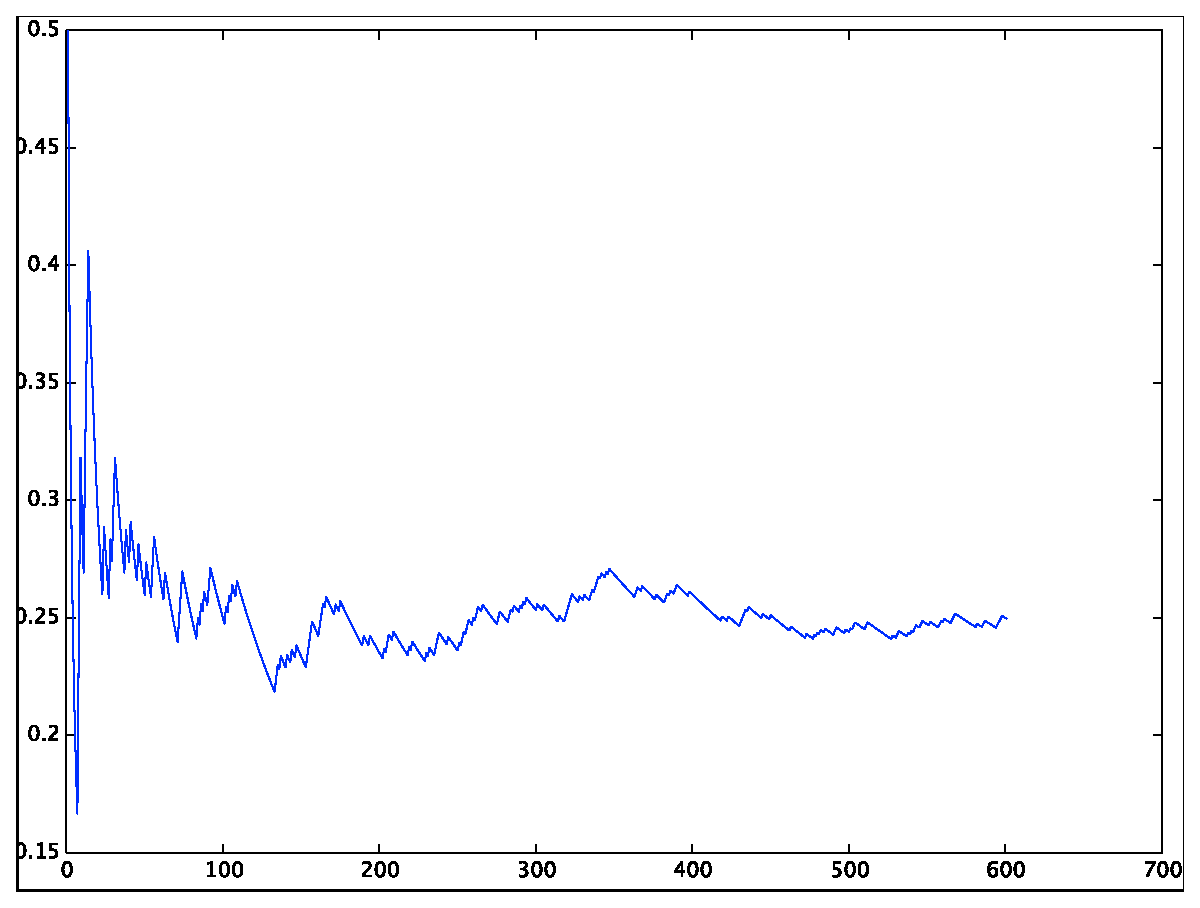
\includegraphics[width=0.7\textwidth]{polyaf1.eps}
  \caption{Grafica 1}
  \label{fig:ejemplo}
\end{figure}

Este c\'odigo esta ejecutando la martingala de las urnas de polya que estuvimos trabajando en clase. Ah\'i probamos que la proporci\'on de bolas rojas es una martingala, adem\'as por el teorema de convergencia de martingalas y dado que polya es una martingala positiva, se  concluye que la martingala converge. En efecto, la simulaci\'on  nos muestra que la proporci\'on de bolas se va estabilizando y por tanto para cada trayectoria que generamos converge. Despu\'es vimos que esta martingala converge a una variable aleatoria con distribuci\'on Beta.



\begin{problema}[Ejercicios sueltos sobre martingalas]
\mbox{}\begin{enumerate}
\item Sea $\paren{X_n,n\geq 0}$ una sucesi\'on $\paren{\F_n}$-adaptada. Pruebe que\begin{esn}
\sum_{k=1}^n X_k-\espc{X_k}{\F_{k-1}}, \quad n\geq 0
\end{esn}es una $\paren{\F_n}$-martingala.
\begin{proof}  Verificamos las tres propiedades para una martingala\\
\begin{itemize}
 	\item Como $\sum_{k=1}^n X_k$ es  $\F_n$- medible y como $\sum_{k=1}^n X_k\espc{X_k}{\F_{k-1}}$ es $\F_{n-1}$-medible, se sigue entonces que  $\sum_{k=1}^n X_k-\espc{X_k}{\F_{k-1}}$ es $\F_n$-medible (Recordar que $\F_{n-1} \subseteq \F_n$)
	\item Suponiendo que  $\paren{X_n,n\geq 0}\in L_1$ se sigue entonces que
	$$
	\esp{\abs{\sum_{k=1}^n X_k-\espc{X_k}{\F_{k-1}}}}\leq \sum_{k=1}^n\esp{ \abs{X_k}} + \esp{\abs{\espc{X_k}{\F_{k-1}}}} 
	$$
	Pero utilizando la desigualdad de Jensen para esperanza condicional $$\abs{\espc{X_k}{\F_{k-1}}} \leq \espc{\abs{X_k}}{\F_{k-1}}$$
	Donde tomando esperanzas tenemos:
	$$
	\esp{\abs{\espc{X_k}{\F_{k-1}}}} \leq \esp{\espc{\abs{X_k}}{\F_{k-1}}}=\esp{\abs{X_k}}
	$$
	Por lo tanto:
	$$
	\esp{\abs{\sum_{k=1}^n X_k-\espc{X_k}{\F_{k-1}}}} \leq \sum_{k=1}^n\esp{ \abs{X_k}} + \esp{\abs{X_k}}
	$$
	Lo que concluye que:
	$$
	\sum_{k=1}^n X_k-\espc{X_k}{\F_{k-1}} \in L_1
	$$
	\item Definamos:$$M_n=\sum_{k=1}^n X_k-\espc{X_k}{\F_{k-1}}$$ queremos probar que $\espc{M_{n+1}}{\F_{n}}=M_{n}$. Veamos:
	$$
	\espc{M_{n+1}}{\F_{n}}=\espc{\sum_{k=1}^{n+1} X_k-\espc{X_k}{\F_{k-1}}}{\F_{n}}
	$$	
	$$
	=\espc{\sum_{k=1}^n X_k-\espc{X_k}{\F_{k-1}}+X_{n+1}-\espc{X_{n+1}}{\F_n}}{\F_{n}}
	$$
	$$
	=M_n+\espc{X_{n+1}}{\F_n}-\espc{X_{n+1}}{\F_n}=M_n
	$$
	Por lo tanto $M_n$ es en efecto una martingala.
\end{itemize}
\end{proof}
\item{Descomposici\'on de Doob para submartingalas}: Sea Sea \(X=\paren{X_n}_{n\in\na}\) una submartingala. Pruebe que \(X\) se puede descomponer de manera \'unica como \(X=M+A\) donde \(M\) es una martingala y \(A\) es un proceso previsible con \(A_0=0\). Sugerencia: Asuma que ya tiene la descomposici\'on y calcule esperanza condicional de \(X_{n+1}\) dada \(X_n\). 
\begin{proof} Para la prueba utilizamos el ejercicio anterior. Como \(X=\paren{X_n}_{n\in\na}\) es un proceso $\F_n$-medible y en $L_1$ entonces usando (1) podemos construir una martingala
$$
M_n=\sum_{k=1}^n X_k-\espc{X_k}{\F_{k-1}}
$$
Suponiendo que tenemos la descomposici\'on $X_n=M_n+A_n$  entonces:
$$
X_n=\sum_{k=1}^n X_k-\espc{X_k}{\F_{k-1}}+A_n
$$
Abriendo la suma (solo el \'ultimo sumando)
$$
X_n=\sum_{k=1}^{n-1} X_k-\espc{X_k}{\F_{k-1}}+X_{n}-\espc{X_{n}}{\F_{n-1}}+A_n
$$
De donde podemos despejar $A_n$, observe que $X_n$ se elimina de la ecuaci\'on anterior.
$$
A_n=\espc{X_{n}}{\F_{n-1}}-\sum_{k=1}^{n-1} X_k-\espc{X_k}{\F_{k-1}}
$$
Notemos que tanto  $\espc{X_{n}}{\F_{n-1}}$ como  $\sum_{k=1}^{n-1} X_k-\espc{X_k}{\F_{k-1}}$ son $\F_{n-1}$-medibles, por lo tanto $A_n$ es predecible y por tanto por construcci\'on se tiene que $X_n=M_n+A_n$. ($A_0:=0$).\\
Observacion: Tomando esperanza a $A_n$ se tiene:
$$
\esp{A_n}=\esp{\espc{X_{n}}{\F_{n-1}}-\sum_{k=1}^{n-1} X_k-\espc{X_k}{\F_{k-1}}}=\esp{X_n}
$$
Como $X_n$ es submartingala entonces sabemos que  $\esp{X_n}$ es creciente conforme $n$ crece por lo tanto $A_n$ es un proceso cuya esperanza tambi\'en es creciente.\\
Ahora probaremos la unicidad, supongamos que existen $M_n^{(1)},M_n^{(2)},A_n^{(1)},A_n^{(2)}$, dos descomposiciones  del proceso $X_n$ es decir:
$$
X_n=M_n^{(1)}+A_n^{(1)}=M_n^{(2)}+A_n^{(2)}
$$
Con $M_n^{(i)}$ martingalas y $A_n^{(i)}$ procesos predecibles, es decir $\espc{A_n^{(i)}}{\F_{n-1}}=A_{n}^{(i)}$.\\
Demostraremos por inducc\'ion que $A_n^{(2)}=A_n^{(1)}$ para toda $n$.\\
Primero para $n=0$, por construcci\'on $A_0^{(1)}=0=A_0^{(2)}$.\\
Supongamos que $A_n^{(1)}=A_n^{(2)}$, por demostrar que $A_{n+1}^{(1)}=A_{n+1}^{(2)}$. 
De la hipotesis  de inducci\'on:  $A_n^{(1)}=A_n^{(2)}$ entonces: $$M_n^{(1)}+A_n^{(1)}=X_n=M_n^{(2)}+A_n^{(2)}$$ De donde se concluye que $M_{n+1}^{(1)}=M_{n+1}^{(2)}$.
$$
A_{n+1}^{(2)}=\espc{A_{n+1}{(2)}}{\F_n}=\espc{X_{n+1}-M_{n+1}^{(2)}}{\F_n}=\espc{X_{n+1}}{\F_{n}}-M_n^{(2)}
$$
$$
=\espc{X_{n+1}}{\F_{n}}-M_n^{(1)}=\espc{M_{n+1}^{(1)}+A_{n+1}^{(1)}}{\F_{n}}-M_n^{(1)}
$$
$$
M_{n}^{(1)}-M_n^{(1)}+\espc{A_{n+1}^{(1)}}{\F_n}=A_{n+1}^{(1)}
$$
Por lo tanto hemos probado que $A_n^{(2)}=A_n^{(1)}$ para toda $n$. Luego se concluye por el hecho de que $X_n=M_n^{(1)}+A_n^{(1)}=M_n^{(2)}+A_n^{(2)} \Rightarrow M_{n}^{(1)}=M_{n}^{(2)}$ para toda $n$. Lo que demuestra la unicidad.
 
\end{proof}


\item Sea \(S_n=\xi_1+\cdots+\xi_n\) donde las variables \(\xi\) son independientes y \(\xi_i\) tiene media cero y varianza finita \(\sigma_i^2\). Pruebe que si \(\sum_i \sigma_i^2<\infty\) entonces \(S_n\) converge casi seguramente y en \(L_2\) conforme \(n\to\infty\). Construya un ejemplo de variables aleatorias \(\xi_i\) tales que la serie \(\sum_i \xi_i\) sea casi seguramente absolutamente divergente y casi seguramente condicionalmente convergente (considere ejemplos simples!). Explique heur\'isticamente por qu\'e cree que suceda esto.
\begin{proof}
Para la prueba utilizamos el teorema 1.6 de las notas. Para ello tenemos que probar que $\esp{\abs{S_n^2}}=\esp{S_n^2}\leq \infty$.\\
Como $\esp{\xi_i}=0$ entonces $\esp{S_n}=0$ de donde concluimos que var$(S_n)=\esp{S_n^2}$. Entonces:
$$
\esp{S_n^2}=var(S_n)=\sum_{i=1}^{n}var(\xi_i)=\sum_{i=1}^{n}\sigma_i^2\leq\sum_{i=1}^{\infty}\sigma_i^2< \infty
$$
Se sigue entonces que por ser $S_n$ martingala, y por el hecho de que  $\esp{\abs{S_n^2}}=\esp{S_n^2}< \infty$ usando Teorema 1.6. $S_n$ converge casi seguramente y en $L_2$  conforme  $n$ tiende a infinito. \\
Ejemplo:
Sea $\xi$ v.a.i.i.d tal que $\p(\xi_i=1)=1/2$ y $\p(\xi_i=-1)=1/2$, entonces $\esp{\xi_i}=0$ y  $var(\xi_i)=1$.Definimos:
$$
S_n=\sum_{i=1}^{n}\frac{\xi_i}{i} \Rightarrow S_{\infty}=\sum_{i=1}^{\infty}\frac{\xi_i}{i}
$$
La serie de la derecha no converge absolutamente pues $\abs{\frac{\xi_i}{i}}=\frac{1}{i}$ (obtenemos la serie armonica). Sin embargo como:
$$
\esp{S_n^2}=var(S_n)=\sum_{i=1}^{n}var\paren{\frac{\xi_i}{i}}=\sum_{i=1}^{n}\frac{1}{i^2}=\frac{\pi^2}{6} < \infty
$$
Se sigue, que aplicando Teorema 1.6 que $S_n$es seguramente condicionalmente convergente.
\end{proof}
%Ser\'a que \sum_i\abs{x_i}=\infty casi seguramente si \sum_i\abs\esp{\xi_i}=\infty? 
\item Sean \(X\) y \(Y\) dos martingalas (respecto de la misma filtraci\'on) y tales que \(\esp{X_i},\esp{Y_i}<\infty\) para toda \(i\). Pruebe la siguiente f\'ormula de integraci\'on por partes: $$ \esp{X_nY_n}-\esp{X_0Y_0}=\sum_{i=1}^n \esp{\paren{X_i-X_{i-1}}\paren{Y_i-Y_{i-1}}} . $$
\begin{proof}
Partimos  del lado derecho:
$$
\paren{X_i-X_{i-1}}\paren{Y_i-Y_{i-1}}=X_iY_i-X_{i}Y_{i-1}-X_{i-1}Y_{i}+X_{i-1}Y_{i-1}
$$
Sumando un cero $X_{i-1}Y_{i-1}-X_{i-1}Y_{i-1}$
$$
=X_iY_i-X_{i-1}Y_{i-1}+\paren{X_{i-1}-X_i}Y_{i-1}+X_{i-1}\paren{Y_{i-1}-Y_i}
$$
Sumando desde $i=1,2...n$ y notando que el primer termino de la ecuaci�\'on anterior es una suma telesc\'opica tenemos:
$$
\sum_{i=1}^{n}\paren{X_i-X_{i-1}}\paren{Y_i-Y_{i-1}}=X_nY_n-X_0Y_0+\sum_{i=1}^{n}\paren{X_{i-1}-X_i}Y_{i-1}+\sum_{i=1}^{n}X_{i-1}\paren{Y_{i-1}-Y_i}
$$
Tomando esperanza  en la igualdad anterior y notando que:
$$
\esp{\paren{X_{i-1}-X_i}Y_{i-1}}=\esp{\espc{\paren{X_{i-1}-X_i}Y_{i-1}}{\F_{i-1}}}=0
$$
$$
\esp{X_{i-1}\paren{Y_{i-1}-Y_i}}=\esp{\espc{X_{i-1}\paren{Y_{i-1}-Y_i}}{\F_{i-1}}}=0
$$
 Se obtiene entonces:
 $$
\esp{ \sum_{i=1}^n \paren{X_i-X_{i-1}}\paren{Y_i-Y_{i-1}}}= \esp{X_nY_n}-\esp{X_0Y_0}
 $$
 De donde por linealidad de la esperanza se obtiene el resultado.
\end{proof}


\item{Desigualdad de Azema-Hoeffding, tomado de \cite[E14.2, p.237]{MR1155402}}
        \begin{enumerate}
        \item Muestre que si \(Y\) es una variable aleatoria con valores en \([-c,c]\) y media cero entonces, para \(\theta\in\re\)
                        $$\esp{e^{\theta Y}}\leq\imf{\cosh}{\theta c}\leq \imf{\exp}{\frac{1}{2}\theta^2c^2}. $$
                        \begin{proof}
                        	Primero probaremos la desigualdad: $\esp{e^{\theta Y}}\leq\imf{\cosh}{\theta c}$.
			Hagamos notar que $f(y)=e^{\theta Y}$ es una func\'ion convexa y por tanto la recta que une a los punto $(-c,e^{\theta Y})$  y $(c,e^{\theta Y})$ est\'a siempre 
			por arriba de la funci\'on $f(y)$. Esto se traduce en la siguiente desigualdad:
			$$
			e^{\theta Y}\leq \frac{e^{c\theta}-e^{-c\theta}}{2c}(Y+c)-e^{-c\theta} \leq \frac{e^{c\theta}-e^{-c\theta}}{2c}(Y+c)
			$$
			La anterior desigualdad se vale para todo $Y(\omega)$ en el intervalo cerrado $[-c,c]$. Luego tomado esperanzas y recodando que por hip�tesis $\esp{Y}=0$ 					obtenemos que:
			$$
			\esp{e^{\theta Y}}\leq \frac{e^{c\theta}-e^{-c\theta}}{c}:=\cosh{\theta c}
			$$ 
			Para la segunda desigualdad solo tenemos que probar que para toda $x$ se tiene   $ \cosh{x} \leq e^{\frac{1}{2}x^2}$. Para ello utilizaremos la descomposici\'on en 				series de la funci\'on $e^x$
			$$
			\cosh{x}:=\frac{1}{2}\paren{e^{x}-e^{-x}}=\frac{1}{2}\paren{\sum_{k=0}^{\infty}\frac{x^k}{k!}-\sum_{k=0}^{\infty}(-1)^k\frac{x^k}{k!}}=\frac{1}{2}\paren{\sum_{k=0}^{\infty}��				\frac{x^k}{k!}}\paren{1-(-1)^k}	
			$$
			La ultima suma solo es valida para numero pares, por lo que la podemos expresar de la siguiente forma
			$$
			\frac{1}{2}\paren{\sum_{k=0}^{\infty}\frac{2x^{2k}}{(2k)!}}=\sum_{k=0}^{\infty}\frac{x^{2k}}{(2k)!}\leq \sum_{k=0}^{\infty}\frac{(\frac{x^2}{2})^k}{(k)!}=e^{\frac{1}{2}x^2}
			$$
			Observacion, la ultima desigualdad es valida por el hecho de que $$(2k)!\leq 2^kk!$$  Esto \'ultimo lo demostraremos por inducci\'on. \\
			Para $k=1$ se tiene $2\leq 2$ por lo tanto es v\'alida\\
			Supongamos que es v\'alida para $k$ por demostrar que es v\'alida para $k+1$
			$$
			(2(k+1))!=(2k+2)(2k+1)(2k!)\geq^*(2k+2)(2k+1)2^kk!
			$$
			$$
			=2^{k+1}(k+1)!(2k+1)\geq 2^{k+1}(k+1)!  
			$$
			Donde la desigualdad con (*) se debe a la hip\'otesis de inducci\'on. \\
			Finalmente hemos probado entonces que para toda x se tiene que 
			$$
			 \cosh{x} \leq e^{\frac{1}{2}x^2} \Rightarrow  \cosh{(c\theta)} \leq e^{\frac{1}{2}\theta^2 c^2}
			$$
			Lo que muestra la desigualdad.
			
                        \end{proof}
                        
        \item Pruebe que si \(M\) es una martingala nula en $n=0$ tal que para algunas constantes \(\paren{c_n,n\in\na}\) se tiene que
                        $$\abs{M_n-M_{n-1}}\leq c_n\quad\forall n $$
                        entonces, para \(x>0\)
                        $$
                        \proba{\max_{k\leq n} M_k\geq x}\leq \imf{\exp}{\frac{x^2}{2\sum_{k=1}^n c_k^2}}.
                        $$
                       \begin{proof}
                       	En esta parte utilizaremos la proposici\'on 1.4 de la notas que dice que para una sub-martingala $M_n$ se tiene:
			$$
			\lambda\p\paren{\max_{1\leq i \leq n}M_i^+>\lambda} \leq \esp{M_n^+}
			$$
			En nuestro caso $M_n$ es martingala por lo que $e^{\theta M_n}$ es una sub-martingala positiva, aplicando la desigualdad de la proposici\'on anterior a esta 					sub-martingala  y tomando $\lambda = e^{\theta x}$ obtenemos que:
			$$
			 e^{\theta x}\p\paren{\max_{1\leq i \leq n} e^{\theta M_i}> e^{ \theta x}} \leq \esp{ e^{\theta M_n}}
			$$
			Pero como el evento $\set{\max_{1\leq i \leq n} e^{\theta M_i}> e^{\theta x}}=\set{\max_{1\leq i \leq n}  M_i>  x}$. Entonces:
			$$
			\p\paren{\max_{1\leq i \leq n}  M_i>  x} \leq  e^{-\theta x} \esp{ e^{\theta M_n}}
			$$
			Para poder utilizar el ejercicio anterior necesitamos  acotar a la martingala $M_n$ la cual es nula en $n=0$. Como:
			$$
			\abs{M_n}=\abs{\sum_{i=1}^{n}M_i-M_{i-1}}\leq \sum_{i=0}^{n}\abs{M_i-M_{i-1}}\leq\sum_{i=0}^{n}c_i=c^*
			$$
			Entonces $\abs{M_n}$ es acotada por $c^*$ por lo que podemos aplicar la desigualdad del ejercicio anterior
			$$
			 \esp{ e^{\theta M_n}} \leq e^{\frac{1}{2}\theta^2(c^*)^2}
			$$
			Por lo tanto:
			$$
			\p\paren{\max_{1\leq i \leq n}  M_i>  x} \leq  e^{-\theta x} e^{\frac{1}{2}\theta^2(c^*)^2}
			$$
                    	Como lo anterior es v\'alido para todo $\theta>0$ , tomamos $\theta=\frac{x}{(c^*)^2}$.Entonces
			$$
			\p\paren{\max_{1\leq i \leq n}  M_i>  x} \leq  exp\paren{-\frac{1}{2}\frac{x^2}{(c^*)^2}} =exp\paren{\frac{-x^2}{2\paren{\sum_{i=1}^{n}c_i}^2}}
                       	$$
		      \end{proof}
                        
        \end{enumerate}
\end{enumerate}
\end{problema}
\begin{problema}
Sea $S_n=\sum_{i=1}^n X_i$ donde $X_1,X_2,\ldots$ son iid. Sea\begin{esn}
\imf{\phi}{\lambda}=\esp{e^{\lambda S_n}}\in (0,\infty].
\end{esn}
\begin{enumerate}
\item Pruebe que si existen $\lambda_1<0<\lambda_2$ tales que $\imf{\phi}{\lambda_i}<\infty$ entonces $\imf{\phi}{\lambda}<\infty$ para toda $\lambda\in [\lambda_1,\lambda_2]$. Sugerencia: escriba $\lambda=a\lambda_1+(1-a)\lambda_2$ para alg\'un $a\in [0,1]$ y aplique la desigualdad de H\"older. A partir de ahora se asume la premisa de este inciso.
\begin{proof}
Supongamos que existen $\lambda_1,\lambda_2$ con la condiciones dadas arriba, entonces usando la sugerencia expresamos a  $\lambda \in [\lambda_1,\lambda_2]$ como: $$\lambda=a\lambda_1+(1-a)\lambda_2$$. Entonces podemos escribir a $\phi(\lambda)$ como sigue:
$$
\phi(\lambda)=\esp{e^{a\lambda_1+(1-a)\lambda_2}}=\esp{e^{a\lambda_1S_n}e^{(1-a)\lambda_2S_n}}
$$
Usando holder con $p=\frac{1}{a}$ y $q=\frac{1}{1-a}$ tenemos:
$$
\esp{e^{a\lambda_1S_n}e^{(1-a)\lambda_2S_n}}\leq \esp{e^{\lambda_1S_n}}^a\esp{e^{\lambda_2S_n}}^{1-a}=\phi(\lambda_1)^a\phi(\lambda_2)^{1-a}
$$
Luego como por hip\'otesis  $\imf{\phi}{\lambda_i}<\infty$  tenemos que 
$$
\phi(\lambda)\leq \phi(\lambda_1)^a\phi(\lambda_2)^{1-a} < \infty
$$
\end{proof}
\item Pruebe que $\esp{\abs{S_n}^k}<\infty$ para toda $k\geq 0$. 
\begin{proof}
Sea $\lambda \in [\lambda_1,\lambda_2]$  con $\lambda\neq 0$ entonces por inciso anterior aseguramos que $\phi(\lambda)< \infty$  y $\phi(-\lambda)< \infty$. Ahora expresamos como serie de taylor a $e^{\abs{\lambda S_n}}$. Entonces:
$$
e^{\abs{\lambda S_n}}=\sum_{k=0}^{\infty}\frac{\abs{\lambda S_n}^k}{k!}
$$
Como $T_m=\sum_{k=0}^{m}\frac{\abs{\lambda S_n}^k}{k!}$ es una sucesi\'on creciente, pues estamos sumando n\'umeros positivos, se tiene  por el teorema de la convergencia mon\'otona que:
$$
\esp{e^{\abs{\lambda S_n}}}=\esp{\lim_{m \rightarrow \infty}T_m}=\lim_{m \rightarrow \infty}\esp{T_m}=\sum_{k=0}^{\infty}\frac{\abs{\lambda}^k \esp{\abs{S_n}^k}}{k!}
$$
Pero como:
$$
\esp{e^{\abs{\lambda S_n}}}=\esp{e^{\lambda S_n}\mathds{1}_{\set{\lambda S_n \geq 0}}}+\esp{e^{-\lambda S_n}\mathds{1}_{\set{\lambda S_n <0}}}
$$
$$
\leq \esp{e^{\lambda S_n}}+\esp{e^{-\lambda S_n}}=\phi(\lambda)+\phi(-\lambda) < \infty
$$
Por lo tanto 
$$
\sum_{k=0}^{\infty}\frac{\abs{\lambda}^k \esp{\abs{S_n}^k}}{k!}\ < \infty
$$
De donde concluimos que:
$$
 \esp{\abs{S_n}^k} < \infty 	\text{ para toda k}
$$
 
\end{proof}

\item Sea $M^\lambda_t=e^{\lambda S_t}/\imf{\phi}{\lambda}$. Argumente que si $M^n$ es el proceso dado por\begin{esn}
M^n_t=\left.\frac{\partial^n}{\partial \lambda^n}\right|_{\lambda=0}M^\lambda_t,
\end{esn}entonces $M^n$ es una martingala para toda $n$. 
\begin{proof}
Para probar esto hay que mostrar que el operador derivada puede salir de la esperanza condicional. La prueba la haremos por inducci\'on sobre $n$. \\Para  $n=1:$\\
Primero recordemos que por la pregunta 1 de la tarea 2 inciso 1) que $M_t^\lambda$ es martingala para toda $\lambda$. Ahora procedamos a verificar que la primera derivada tambi\'en es martingala para toda $\lambda$, en particular para $\lambda=0$. Como:
$$
\espc{\frac{\partial^1}{\partial \lambda^1}M^\lambda_t}{\F_{t-1}}*=\frac{\partial^1}{\partial \lambda^1}\espc{M^\lambda_t}{\F_{t-1}}
$$
Como $M_t^\lambda$ es martingala   se sigue que:
$$
\frac{\partial^1}{\partial \lambda^1}\espc{M^\lambda_t}{\F_{t-1}}=\frac{\partial^1}{\partial \lambda^1}M^{\lambda}_{t-1}
$$
Por lo que hemos probado que en efecto la derivada   tiene la propiedad de martingala, en particular, evaluando en $\lambda=0$ se tendr\'ia que $M^1_t$ tiene la propiedad de martingala, adem\'as como:
$$
\frac{\partial^1}{\partial \lambda^1}M_t^{\lambda}=\lim_{n \rightarrow \infty}n\paren{M_t^{\lambda+\frac{1}{n}}- M_t^{\lambda}}
$$ 
Se sigue que $M_t^1$ es limite de funciones $\F_t$ medibles y por lo tanto $M_t^1$ es  $\F_t$ medible. \\
(*)Note que en la prueba se est\'a haciendo uso de que podemos intercambiar esperanza con derivada.\\
Ahora supongamos que $\frac{\partial^{n}}{\partial \lambda^{n}}M^\lambda_t$ es martingala, y demostrarmos que $\frac{\partial^{n+1}}{\partial \lambda^{n+1}}M^\lambda_t$ es martingala.
Tenemos lo siguiente:
$$
 \espc{\frac{\partial^{n+1}}{\partial \lambda^{n+1}}M^\lambda_t}{\F_{t-1}}*=\frac{\partial^1}{\partial \lambda^1}\espc{\frac{\partial^{n}}{\partial \lambda^{n}}M^\lambda_t}{\F_{t-1}}=
\frac{\partial^1}{\partial \lambda^1}\frac{\partial^{n}}{\partial \lambda^{n}}M^\lambda_{t-1}
$$
Donde la ultima igualdad es por la hip\'otesis de inducci\'on adem\'as de  que nuevamente estamos haciendo uso de que  en la esperanza condicional se puede introducir la derivada. Finalmente se tiene que;
$$
 \espc{\frac{\partial^{n+1}}{\partial \lambda^{n+1}}M^\lambda_t}{\F_{t-1}}=\frac{\partial^{n+1}}{\partial \lambda^{n+1}}M^\lambda_{t-1}
$$
En particular, evaluando $\lambda=0$ obtenemos que en efecto $M_t^{n+1}$ es martingala y por la inducci\'on se sigue que esto es v\'alido para toda $n$.\\Sin embargo para que esta prueba sea v\'alida hay que probar que en efecto estamos en condiciones de  sacar la derivada de la esperanza condicional. A continuaci\'on presento una prueba  parcial de este hecho:\\
Queremos mostrar que bajo la condiciones de nuestro problema se tiene:
$$
\espc{\frac{\partial^1}{\partial \lambda^1}M^\lambda_t}{\F_{t-1}}*=\frac{\partial^1}{\partial \lambda^1}\espc{M^\lambda_t}{\F_{t-1}}
$$
El prueba consistir\'a en utilizar el T.C.D. para la esperanza condicional, es decir utilizaremos el teorema que nos indica  que si $\paren{X_n}$ es una sucesi\'on  de variables  en $L_1$ puntualmente convergente y existe $Y$ integrable tal que $\abs{X_n}\leq Y$ para $n\in \mathds{N} $ entonces:
$$
\espc{\lim_{n \rightarrow \infty}X_n}{\G}=\lim_{n \rightarrow \infty}\espc{X_n}{\G}
$$
En nuestro caso definiremos  lo siguiente:
$$
X_n=n\paren{M_t^{\lambda+\frac{1}{n}}-M_t^{\lambda}} \rightarrow_{n \rightarrow \infty} X=\frac{\partial^1}{\partial \lambda^1}M^\lambda_t
$$
Si mostramos que $X_n$ es dominada por una una variable Y integrable ya acabamos pues por el T.C.D para  la esperanza condicional nos dir�a que;
$$
\espc{\frac{\partial^1}{\partial \lambda^1}M^\lambda_t}{\G}=\espc{\lim_{n \rightarrow \infty}X_n}{\G}=\lim_{n \rightarrow \infty}\espc{X_n}{\G}
$$
Pero 
$$
\lim_{n \rightarrow \infty}\espc{X_n}{\G}=\lim_{n \rightarrow \infty}\espc{n\paren{M_t^{\lambda+\frac{1}{n}}-M_t^{\lambda}}}{\G}
$$
$$
=\lim_{n \rightarrow \infty}n\paren{\espc{M_t^{\lambda+\frac{1}{n}}}{\G}- \espc{M_t^{\lambda}}{\G}  }=\frac{\partial^1}{\partial \lambda^1}\espc{M^\lambda_t}{\G}
$$
Ahora hay que mostar que en efecto podemos dominar a $X_n$. Bajo el supuesto de que $\abs{\frac{\partial^1}{\partial \lambda^1}M^\lambda_t} < m(\omega)$ donde $m:\Omega \rightarrow \mathds{R}$ es integrable se tendri\'a que: 
$$
\abs{X_n}=n\abs{\paren{M_t^{\lambda+\frac{1}{n}}-M_t^{\lambda}}}=n\abs{\int_{\lambda}^{\lambda+\frac{1}{n}}\frac{\partial^1}{\partial \lambda^1}M^\lambda_t d\lambda  } \leq
n\int_{\lambda}^{\lambda+\frac{1}{n}}\abs{\frac{\partial^1}{\partial \lambda^1}M^\lambda_t} d\lambda  
$$
$$
\leq  n\int_{\lambda}^{\lambda+\frac{1}{n}} m(\omega) d\lambda  = m(\omega)n\paren{\lambda +\frac{1}{n}-\lambda}=m(\omega) 
$$
Y como la funci\'on $m(\omega)$ la suponemos integrable, entonces se sigue la sucesi\'on es dominada por una  variable integrable y podemos aplicar T.D.C para esperanza condicional.\\
Obs: (No pude encontrar una cota para  la primera derivada: $\abs{\frac{\partial^1}{\partial \lambda^1}M^\lambda_t} $ :(

\end{proof}
\item Calcule las primeras $4$ martingalas resultantes si $\proba{X_i=\pm 1}=1/2$. Util\'icelas para calcular el valor de $\esp{T^2}$ donde\begin{esn}
T=\min\set{n\geq 0: S_n\in\set{-a,b}}
\end{esn}y $a,b>0$. 
\begin{proof}
Derivando y evaluando en $\lambda=0$, y recordando que estamos bajo la hip\'otesis de que $\phi(\lambda)$ esta acotada en una vecindad del cero tenemos que:
$$
\left.\frac{\partial^{(k)}}{\partial \lambda^{k}}\right|_{\lambda=0} \phi(\lambda)=\left.\esp{\frac{\partial^{(k)}}{\partial \lambda^{k}} \right|_{\lambda=0}e^{\lambda S_n}}=\esp{S_n^k} < \infty
$$
Esto quiere decir que las derivadas de $\phi(\lambda)$ evaluadas en 0 nos proporcionan los distintos momentos de $S_n$.Ademas dado que estamos en una caminata aleatoria donde $\proba{X_i=\pm 1}=1/2$. Entonces:
$$\esp{S_n}=0=\left.\frac{\partial^{(1)}}{\partial \lambda^{1}}\right|_{\lambda=0} \phi(\lambda)$$$$\esp{S_n^2}=n=\left.\frac{\partial^{(2)}}{\partial \lambda^{2}}\right|_{\lambda=0} \phi(\lambda)$$$$\esp{S_n^3}=0=\left.\frac{\partial^{(3)}}{\partial \lambda^{3}}\right|_{\lambda=0} \phi(\lambda)$$$$\esp{S_n^4}=3n^2-2n=\left.\frac{\partial^{(4)}}{\partial \lambda^{4}}\right|_{\lambda=0} \phi(\lambda)$$
Las martingalas que obtenemos son las siguientes:
\begin{enumerate}
	\item$$M^1_t=\left.\frac{\partial^1}{\partial \lambda^1}\right|_{\lambda=0}M^\lambda_t=S_t$$
	\item$$M^2_t=\left.\frac{\partial^2}{\partial \lambda^2}\right|_{\lambda=0}M^\lambda_t=S_t^2-t$$
	\item$$M^3_t=\left.\frac{\partial^3}{\partial \lambda^3}\right|_{\lambda=0}M^\lambda_t=S_t^3-3tS_t$$
	\item$$M^4_t=\left.\frac{\partial^4}{\partial \lambda^4}\right|_{\lambda=0}M^\lambda_t=S_t^4-6tS_t^2+3t^2+2t$$
\end{enumerate}

Luego como vimos en clase  $S_T$ (La caminata evaluada en el tiempo de paro) es una variable que toma dos valores :
$$
\p(S_T=-a)=\frac{b}{a+b}
$$
$$
\p(S_T=b)=\frac{a}{a+b}
$$
Entonces 
$$\esp{S_T}=0$$
$$\esp{S_T^2}=ab$$
$$\esp{S_T^3}=ab(a-b)$$
$$\esp{S_T^4}=\frac{ab(a^3+b^3)}{a+b}$$
Luego, usando el muestro opcional de Doob y dado que todas las martingalas generadas tiene media cero obtenemos que;
$$
0=\esp{S_T^4-6TS_T^2+3T^2+2T}=\esp{S_T^4}-6\esp{TS_T^2}+3\esp{T^2}+2\esp{T}
$$ 
De donde despejando:
$$
\esp{T^2}=\frac{6\esp{TS_T^2}-\frac{ab(a^3+b^3)}{a+b}-2ab}{3}
$$
*Falta evaluar $\esp{TS_T^2}=?$\\
Solucionaremos el problema para el caso en que $a=b$. \\
Cuando $a=b$ entonces $S_T^2$ solo toma una valor que es $a^2$ por lo que la formula nos queda:
$$
\esp{T^2}=\frac{6\esp{Ta^2}-\frac{ab(a^3+b^3)}{a+b}-2ab}{3}
$$
Simplificando:
$$
\esp{T^2}=\frac{a^2(5a^2-2)}{3}
$$
Con esto ya podemos calcular la varianza de T.
$$
Var(T)=\esp{T^2}-\esp{T}=\frac{a^2(5a^2-2)}{3}-a^2
$$
Llevamos a cabo simulaciones en R para verificar nuestro resultado, a continuaci\'on se presenta la simulaci\'on de $30,000$ caminatas aleatorias donde $a=3$ y $b=3$. El resultado te\'orico nos dice que $\esp{T^2}=129$ mientras que las simulaciones se estabilizaron en un valor de $129.1989$ . A continuaci\'on presentamos c\'odigo y gr\'afica 

\begin{lstlisting}
a=3
b=3
T=0
Sim=30000
for (k in 1:Sim){
  S=0
  S[1]=0
  j=1
  while (((S[j]>-a) && (S[j]<b)) ){
    u=runif(1)
    if (u <= 1/2)  Y=1  else  Y=-1
    S[j+1]=S[j]+Y
    j=j+1
  }
  T[k]=(j-1)^2
}
mean(T)
a^2*(5*a^2-2)/3
\end{lstlisting}
\end{proof}
\begin{figure}
  \centering
    \includegraphics[width=0.7\textwidth]{simula1.jpg}
  \caption{Grafica 1}
  \label{fig:ejemplo}
\end{figure}
\end{enumerate}

\defin{Categor\'ias:} Caminatas aleatorias, muestreo opcional, ejemplos de martingalas. 
\end{problema}

%
%\begin{problema}
%Sean $\F_1,\F_2,\ldots $ y $\G$ sub\sa s de $\F$. Decimos que $\F_1,\F_2,\ldots$ son condicionalmente independientes dada $\G$ si para cualquier $H_i$ que sea $\F_i$ medible y acotada se tiene que\begin{esn}
%\espc{H_1\cdots H_n}{\G}=\espc{H_1}{\G}\cdots \espc{H_n}{\G}.
%\end{esn}
%\begin{enumerate}
%\item ?`Qu\'e quiere decir la independencia condicional cuando $\G=\set{\oo,\emptyset}$?
%\item Pruebe que $F_1$ y $\F_2$ son condicionalmente independientes dada $\G$ (denotado $\condind{\F_1}{\F_2}{\G}$) si y s\'olo si para cualquier $H$ que sea $\F_1$-medible y acotada se tiene que\begin{esn}
%\espc{H}{\F_2,\G}=\espc{H}{\G}.
%\end{esn}
%\item Pruebe que $\F_1,\F_2,\ldots, $ son condicionalmente independientes dada $\G$ si y s\'olo si para cada $n\geq 1$, $\F_{n+1}$ es condicionalmente independiente de $\F_1,\ldots, \F_n$ dada $\G$. 
%\end{enumerate}
%
%\defin{Categor\'ias: } Esperanza condicional, Independencia condicional.
%\end{problema}
%
%\begin{problema}
%Sea $\mu$ una distribuci\'on de progenie y defina $\tilde \mu_j=\mu_{j+1}$. Sea $S=\paren{S_n}$ una caminata aleatoria con distribuci\'on de salto $\tilde\mu$. Sea $k$ un entero no-negativo y defina recursivamente\begin{esn}
%Z_0=k=C_0,\quad Z_{n+1}=k+S_{C_n}\quad\text{y} C_{n+1}=C_n+Z_{n+1}.
%\end{esn}
%\begin{enumerate}
%\item Pruebe que $Z_n\geq 0$ para toda $n$ y que si $Z_n=0$ entonces $Z_{n+1}=0$.
%\item Pruebe que $C_n$ es un tiempo de paro para la filtraci\'on can\'onica asociada a $S$.
%\item Pruebe que $Z$ es un proceso de Galton-Watson con ley de progenie $\mu$. 
%\item Pruebe que si $S$ alcanza $-1$ entonces existe $n$ tal que $Z_n=0$. Deduzca que si la media de $\mu$ es $1$ entonces $Z$ se extingue. (Sugerencia: utilice un ejercicio anterior sobre martingalas con saltos acotados hacia abajo.) 
%\end{enumerate}
%
%\defin{Categor\'ias: } Caminatas aleatorias, Procesos de Galton-Watson%, Propiedad de Markov fuerte.
%\end{problema}
%
%\begin{problema}
%Sea $\mu$ una distribuci\'on de progenie y defina $\tilde \mu_j=\mu_{j+1}$. Sea $\nu$ una distribuci\'on en $\na$. Consideremos a dos caminatas aleatorias $S=\paren{S_n}$  y $T$ con  distribuci\'ones de salto $\tilde\mu$ y $\nu$.
%\begin{enumerate}
%\item ?`Qu\'e significa que $S$ y $T$ sean independientes? As\'umalo.
%\item Sea $k$ un entero no-negativo y defina recursivamente\begin{esn}
%Z_0=k=C_0,\quad Z_{n+1}=k+S_{C_n}+T_n\quad\text{y} C_{n+1}=C_n+Z_{n+1}.
%\end{esn}
%\item Pruebe que $Z_n\geq 0$ para toda $n$.
%\item Pruebe que $C_n=k\in\F^S_k\cap\F^T_n$.
%\item Pruebe que $Z$ es un proceso de Galton-Watson con inmigraci\'on.
%\end{enumerate}
%
%\defin{Categor\'ias: } Caminatas aleatorias, Procesos de Galton-Watson, Construcci\'on de procesos estoc\'asticos
%\end{problema}
%
%\begin{problema} %Construcci\'on tipo Poisson 
%Sean $\mu$ y $\nu$ una distribuci\'on de progenie y de inmigraci\'on. Sean $Y_1,Y_2,\ldots$ independientes y de ley $\nu$. Suponga que condicionalmente a $Y$, $X^0,X^1,X^2,\ldots$ son procesos de Galton-Watson independientes tales que $X^0_0=k$ y $X^k_0=Y_k$ para $k\geq 1$. Pruebe que si\begin{esn}
%Z_n=\sum_{k=0}^n X^k_{n-k},
%\end{esn}entonces $Z$ es un proceso de Galton-Watson con distribuciones de progenie e inmigraci\'on $\mu$ y $\nu$ que comienza en $k$. 
%
%\defin{Categor\'ias: } Procesos de ramificaci\'on
%\end{problema}
%
%\begin{problema}
%Para cada par de medidas de probabilidad en $\na^\na$ $\p_1$ y $\p_2$ definimos a la convoluci\'on de $\p_1$ y $\p_2$, denotada $\p_1 *\p_2$, como la distribuci\'on de $\paren{S^1_k+S^2_k,k\geq 0}$ donde $S^1$ y $S^2$ son independientes y de distribuciones $\p_1$ y $\p_2$ respectivamente.
%\begin{enumerate}
%\item ?` Cu\'al es la relaci\'on entre las distribuciones finito-dimensionales de $\p_1$, $\p_2$ y $\p_1*\p_2$?
%\item Sea $\p_k^\mu$ la distribuci\'on de un proceso de Galton-Watson  de ley de reproducci\'on $\mu$ que comienza en $k$. Pruebe que $\p_{k_1}*\p_{k_2}=\p_{k_1+k_2}$.
%%\item Caracterizaci\'on de leyes markovianas con la propiedad de ramificaci\'on.
%\end{enumerate}
%
%\defin{Categor\'ias: } Distribuciones finito-dimensionales, Procesos de ramificaci\'on.
%\end{problema}
\bibliography{GenBib}
\bibliographystyle{amsalpha}
\end{document}